\subsection{Estado del arte}

Los entornos más destacables que hemos encontrado son los siguientes:
\begin{itemize}
    \item \textbf{Neural MMO} está basado en el género del de gaming MMORPGs (massively multiplayer online role-playing games). Se trata de un gran entorno 3D que contiene diferentes recursos  y los agentes progresan a través de un complejo sistema de progresión. Podemos ver la representación del entorno en la figura \ref{fig:neural-mmo}. Los agentes compiten entre ellos y están restringidos a una observación parcial. \cite{env-list} 
        \begin{figure}[ht]
            \centering
            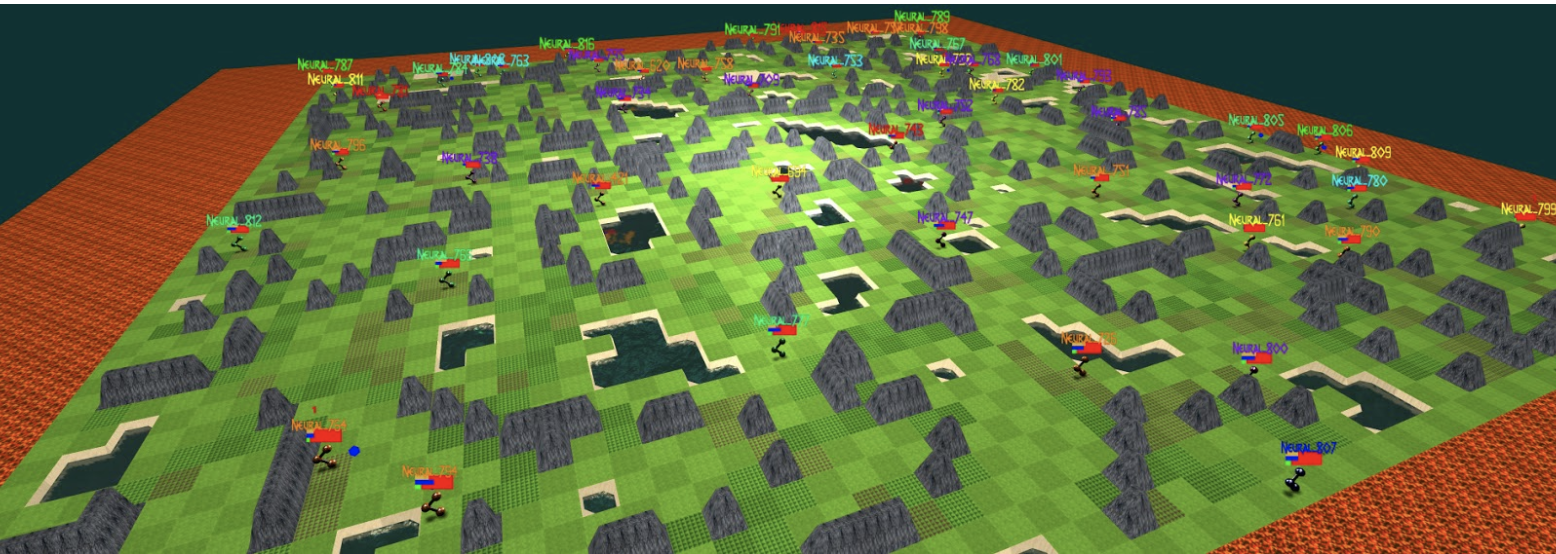
\includegraphics[width=0.7\textwidth]{img/neural-mmo.png}
            \caption{Entorno gráfico 3D de Neural MMO \cite{neural-mmo}}
            \label{fig:neural-mmo}
        \end{figure}
    \item \textbf{PettingZoo} es una librería de Python para realizar investigaciones en MARL. Contiene multiples problemas de este ámbito y sigue la interfaz Gym de OpenIA. Los entornos que incluye son juegos multijugador de Atari 2600, juegos desarrollados por ellos mismos y por parte de terceros. Algunos de ellos contienen tareas simples de comunicación entre agentes.\cite{env-list}
    \item \textbf{MALMO} es un entorno basado en el juego de Minecraft. Su mundo 3D contiene un conjunto muy diverso de tareas y sub entornos. Agentes interactúan con otros agentes y entidades de diversas formas. Además tiene la ventaja de que fue usado en The Malmo Collaborative AI Challenge y esto aportó una gran cantidad de código y nuevos entornos. \cite{env-list} Podemos ver un ejemplo de entorno creado en MALMO en la figura \ref{fig:mob-chase}.
        \begin{figure}[ht]
            \centering
            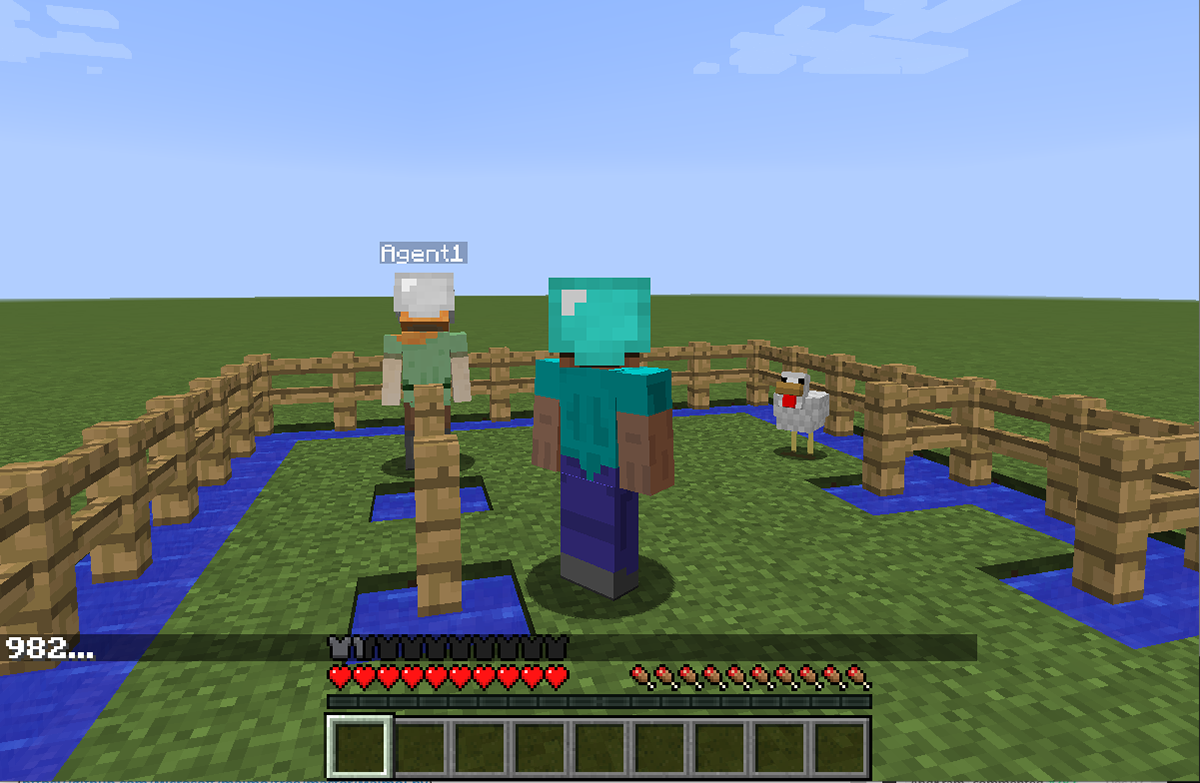
\includegraphics[width=0.5\textwidth]{img/mobchase.png}
            \caption{Entorno gráfico 3D de MALMÖ en Minecraft. Se puede observar la tarea de capturar al animal \cite{malmo}}
            \label{fig:mob-chase}
        \end{figure}
        
    \item \textbf{TrinityCore} es un framework de MMORPG usado principalmente como un simulador de un servidor del conocido videojuego World of Warcraft. Este framework se ha usado en otros trabajos del mismo ámbito como \cite{wow-upc}. Este puede ser adaptado ya que este videojuego tiene mecánicas complejas como el comercio, el uso de roles.
\end{itemize}
